\documentclass[12pt,a4paper]{article}
\usepackage{amsmath,amssymb}
\usepackage{graphicx}
\usepackage{hyperref}
\usepackage{booktabs}
\usepackage{geometry}
\geometry{margin=2.5cm}

\title{\textbf{Threshold Analysis of the Rotated Surface Code\\
Under Depolarizing Noise: A Comparative Study of\\
MWPM and Neural Network Decoders}}
\author{Samkelo Mhlophe\\
Durban University of Technology}
\date{March 2026}

\begin{document}
\maketitle

\begin{abstract}
Quantum error correction (QEC) is a prerequisite for fault-tolerant quantum
computation. This paper presents a Monte Carlo simulation of the rotated surface
code under a depolarizing noise model across code distances $d \in \{3,5,7,9,11\}$,
implemented using the Stim stabilizer simulator. Two decoders are compared:
minimum-weight perfect matching (MWPM) via PyMatching, and a feedforward neural
network (NN) trained on syndrome data. A threshold of approximately
$p_{\text{th}} \approx 0.01$ is identified for MWPM, consistent with theoretical
predictions. The NN decoder performs significantly worse than MWPM at low error
rates due to class imbalance in the training data, motivating future work on
improved learned decoders. Below threshold, MWPM achieves exponential logical
error suppression with increasing code distance.
\end{abstract}

\section{Introduction}
Physical qubits are subject to decoherence, gate imperfections, and environmental
noise. Without error correction, quantum computations cannot proceed beyond a small
number of operations. Quantum error correcting codes protect logical information by
distributing it across multiple physical qubits such that errors can be detected and
corrected without measuring the encoded state directly.

The surface code \cite{kitaev1997} is the leading candidate for fault-tolerant
quantum computation due to its high threshold, local stabilizer measurements, and
compatibility with planar qubit architectures. The rotated surface code
\cite{fowler2012} reduces qubit overhead while preserving error correction properties.

This paper addresses two questions: (1) how does logical error suppression scale
with code distance from $d=3$ to $d=11$ under MWPM decoding, and (2) can a simple
feedforward neural network match MWPM performance as a decoder?

\section{Background}

\subsection{Qubits and Pauli Errors}
A qubit exists in superposition $|\psi\rangle = \alpha|0\rangle + \beta|1\rangle$
where $|\alpha|^2 + |\beta|^2 = 1$. Three independent error types act on qubits:
\begin{align}
X|0\rangle &= |1\rangle, \quad X|1\rangle = |0\rangle \quad \text{(bit-flip)}\\
Z|0\rangle &= |0\rangle, \quad Z|1\rangle = -|1\rangle \quad \text{(phase-flip)}\\
Y &= iXZ \quad \text{(combined bit and phase flip)}
\end{align}

\subsection{Stabilizer Formalism}
A stabilizer code is defined by commuting Pauli operators $\{S_i\}$ whose
simultaneous $+1$ eigenspace defines the code space. When error $E$ anticommutes
with stabilizer $S_i$:
\begin{equation}
S_i(E|\psi\rangle) = -(E|\psi\rangle)
\end{equation}
The eigenvalue flips to $-1$, yielding a classical syndrome bit identifying the
error without collapsing the encoded quantum state.

\subsection{The Rotated Surface Code}
A distance-$d$ rotated surface code encodes one logical qubit in $d^2$ data qubits
with $(d^2-1)/2$ X-stabilizers and $(d^2-1)/2$ Z-stabilizers. The code distance
$d$ is the minimum weight of an undetectable logical error.

\begin{table}[h]
\centering
\caption{Qubit counts for each code distance}
\begin{tabular}{ccc}
\toprule
Distance $d$ & Data Qubits & Total Qubits (with ancilla) \\
\midrule
3 & 9 & 26 \\
5 & 25 & 58 \\
7 & 49 & 106 \\
9 & 81 & 170 \\
11 & 121 & 250 \\
\bottomrule
\end{tabular}
\end{table}

\section{Methodology}

\subsection{Noise Model}
A symmetric depolarizing channel was applied with physical error rate $p$:
\begin{equation}
\mathcal{E}(\rho) = (1-p)\rho + \frac{p}{3}(X\rho X + Y\rho Y + Z\rho Z)
\end{equation}
Two-qubit gates receive a depolarizing channel with per-Pauli probability $p/15$.

\subsection{MWPM Decoder}
Circuits were generated using Stim \cite{gidney2021} with the
\texttt{surface\_code:rotated\_memory\_z} template. Decoding was performed using
PyMatching \cite{higgott2022} via minimum-weight perfect matching on the detector
error model. Each configuration was sampled with $N=100{,}000$ Monte Carlo shots
across 15 logarithmically spaced error rates from $p=10^{-3}$ to $p=10^{-1}$.

\subsection{Neural Network Decoder}
A feedforward neural network was trained to classify syndromes as logical error
or no logical error. Architecture: input layer (syndrome size) $\to$ 128 units
(ReLU) $\to$ 64 units (ReLU) $\to$ 1 unit (Sigmoid). Training used 30,000
syndrome-label pairs per configuration, Adam optimizer, binary cross-entropy loss,
15 epochs. Evaluation used 10,000 held-out shots.

\begin{table}[h]
\centering
\caption{Simulation parameters}
\begin{tabular}{ll}
\toprule
Parameter & Value \\
\midrule
Code distances (MWPM) & $d \in \{3, 5, 7, 9, 11\}$ \\
Code distances (NN) & $d \in \{3, 5, 7\}$ \\
Error correction rounds & 10 \\
MWPM shots & 100,000 per configuration \\
NN training shots & 30,000 per configuration \\
NN evaluation shots & 10,000 per configuration \\
Physical error rate range & $[10^{-3}, 10^{-1}]$ \\
Simulator & Stim v1.15.0 \\
\bottomrule
\end{tabular}
\end{table}

\section{Results}

\subsection{MWPM Threshold Analysis}
Figure \ref{fig:extended} shows logical error rates for $d \in \{3,5,7,9,11\}$.
All curves converge near $p_{\text{th}} \approx 0.01$, confirming the threshold.

\begin{figure}[h]
\centering
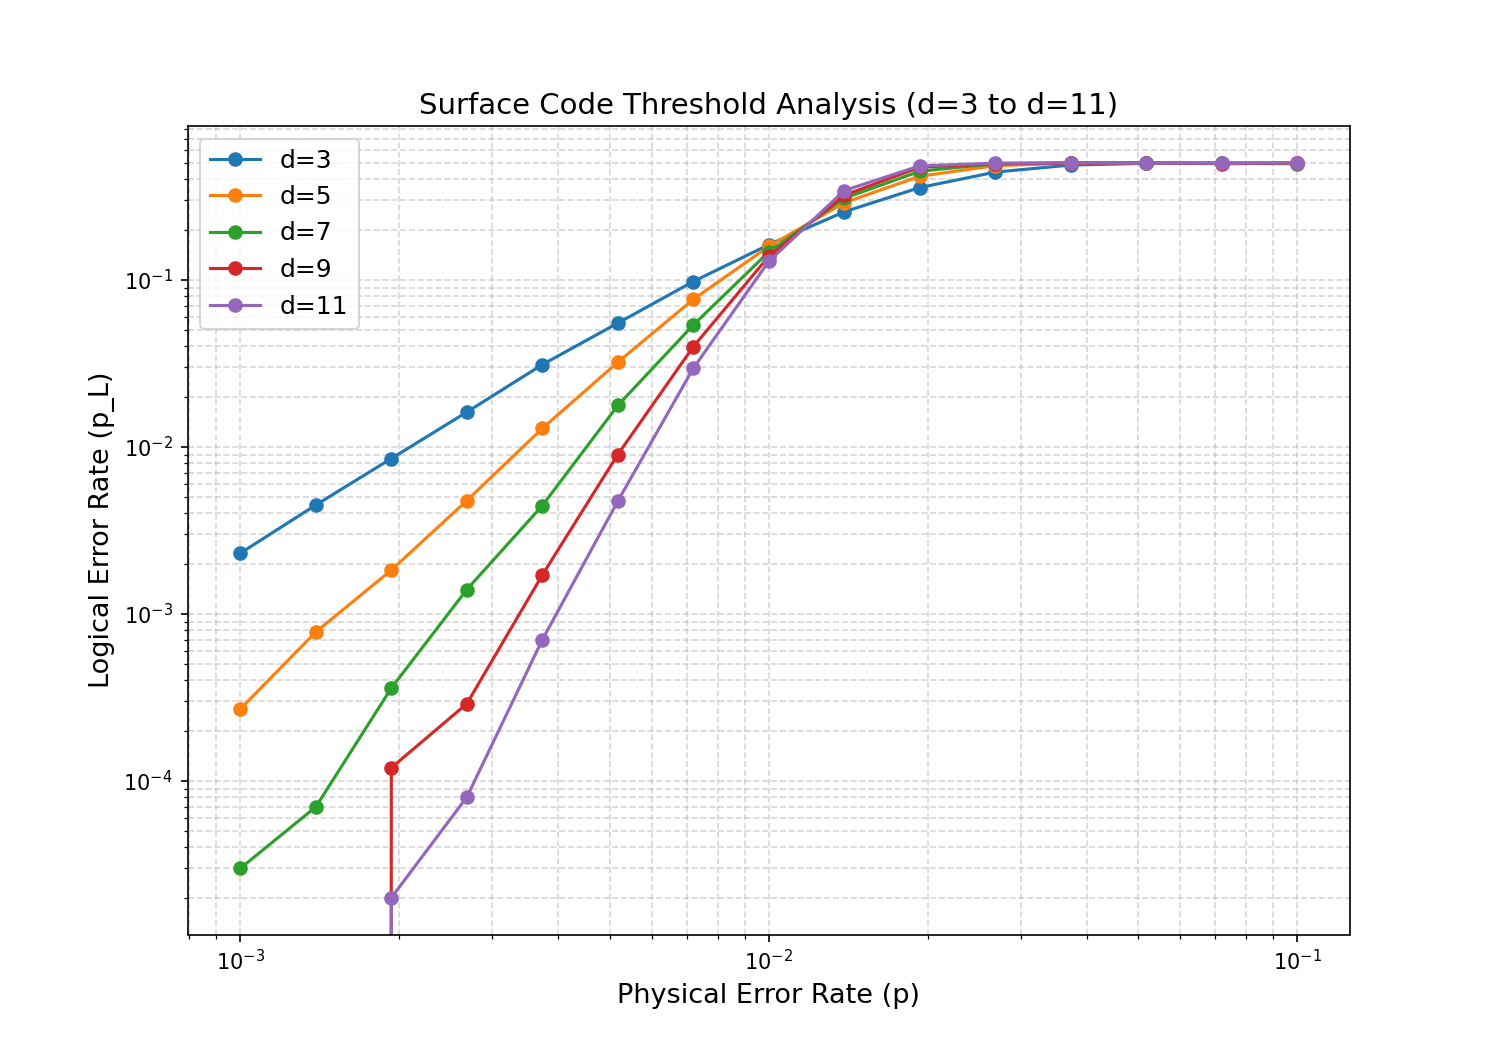
\includegraphics[width=0.85\textwidth]{../figures/threshold_plot_extended.png}
\caption{Logical error rate vs physical error rate for $d \in \{3,5,7,9,11\}$
under MWPM decoding. Curves converge near $p \approx 0.01$.}
\label{fig:extended}
\end{figure}

\subsection{Below-Threshold Scaling}
At $p = 0.001$, logical error rates under MWPM were:

\begin{table}[h]
\centering
\caption{MWPM logical error rates at $p = 0.001$}
\begin{tabular}{ccc}
\toprule
Distance $d$ & $p_L$ & Suppression vs $d=3$ \\
\midrule
3 & 0.00231 & $1\times$ \\
5 & 0.00027 & $8.6\times$ \\
7 & 0.00003 & $77\times$ \\
9 & 0.00000 & $>231\times$ \\
11 & 0.00000 & $>231\times$ \\
\bottomrule
\end{tabular}
\end{table}

Each distance increment of 2 reduces the logical error rate by approximately
one order of magnitude, consistent with the theoretical scaling:
\begin{equation}
p_L \sim \left(\frac{p}{p_{\text{th}}}\right)^{\lfloor(d+1)/2\rfloor}
\end{equation}

\subsection{MWPM vs Neural Network Decoder}
Figure \ref{fig:comparison} compares MWPM and NN decoder performance for
$d \in \{3,5,7\}$.

\begin{figure}[h]
\centering
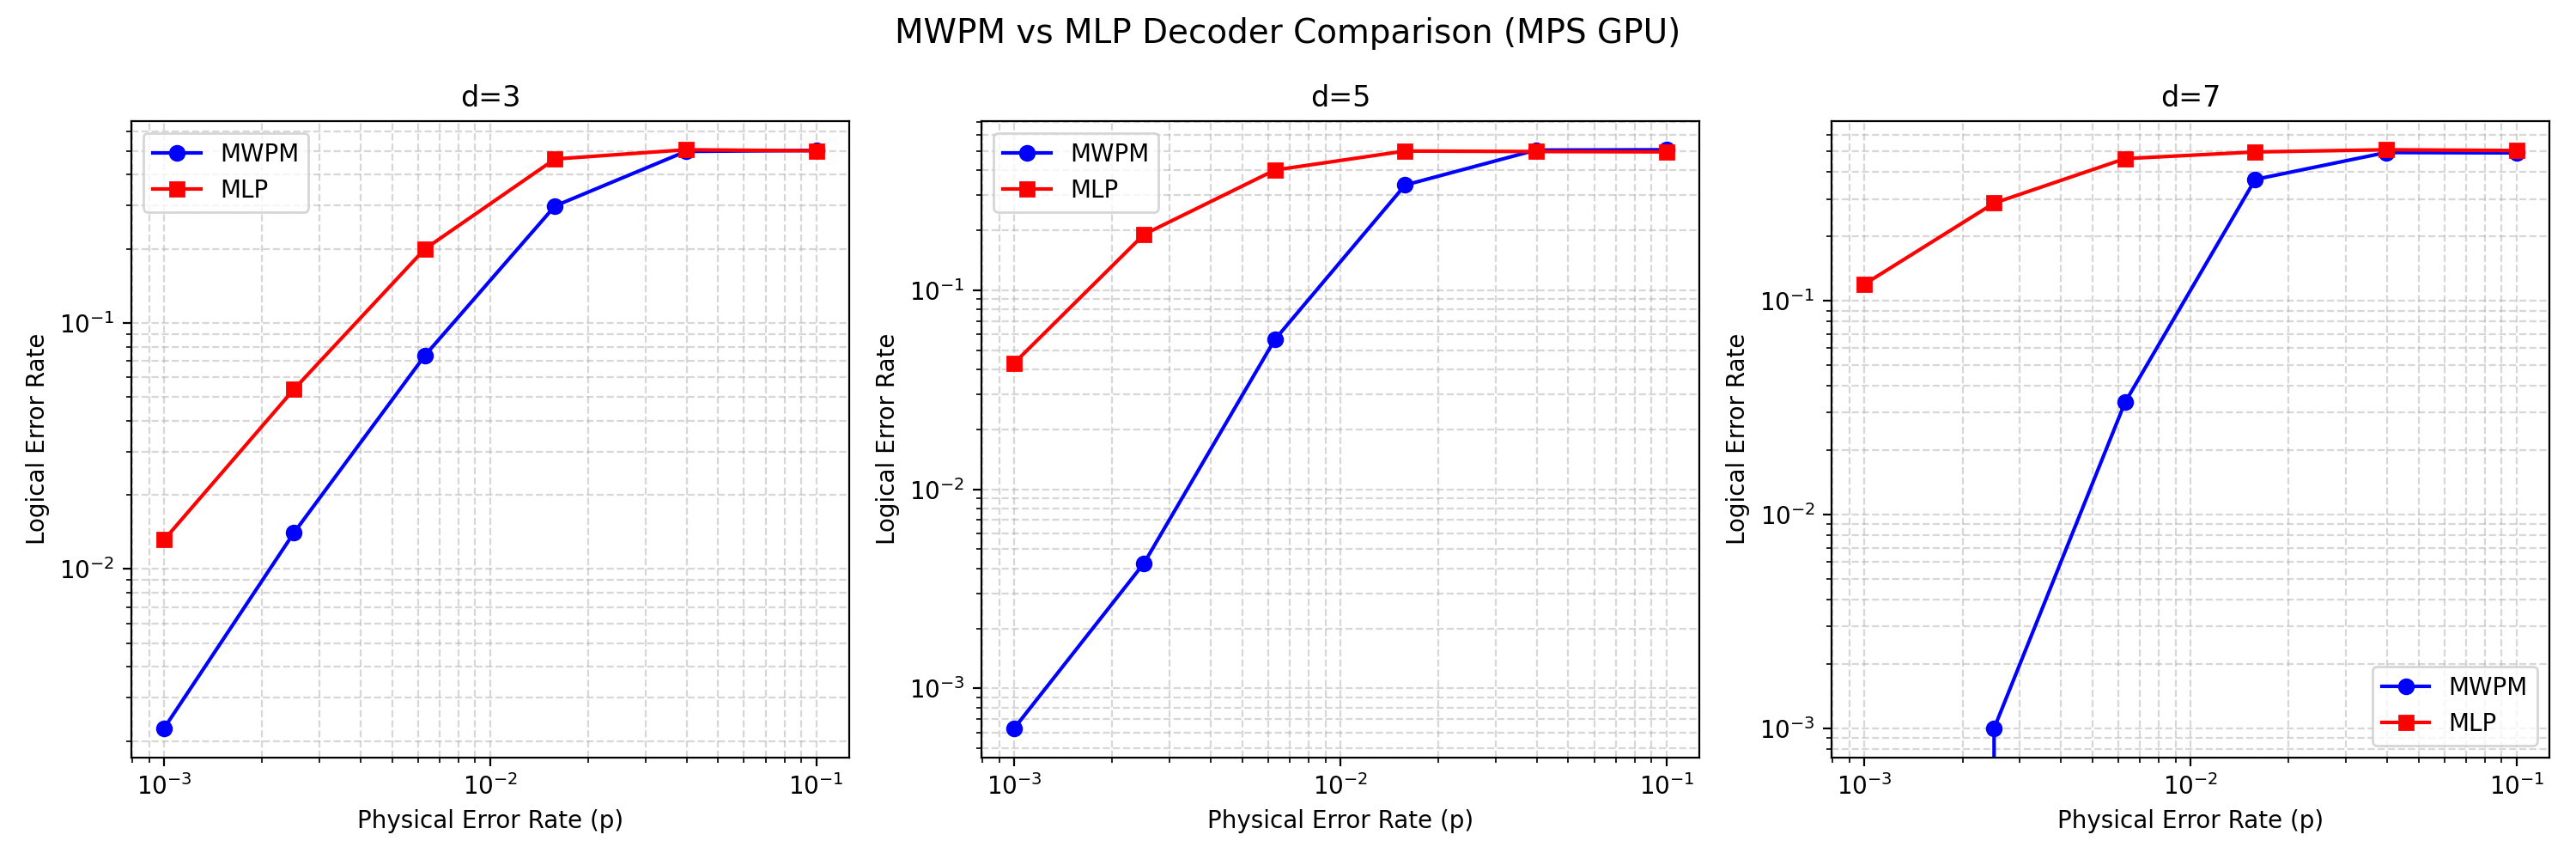
\includegraphics[width=\textwidth]{../figures/decoder_comparison.png}
\caption{MWPM vs neural network decoder logical error rates for $d=3,5,7$.
MWPM consistently outperforms the NN decoder, particularly at low error rates.}
\label{fig:comparison}
\end{figure}

At $p=0.001$ for $d=7$, MWPM achieves $p_L \approx 0$ while the NN decoder
produces $p_L \approx 0.097$. This gap arises from class imbalance: at low
physical error rates, logical errors are rare, providing insufficient positive
training examples for the network to learn the error structure. The NN decoder
converges toward random guessing ($p_L \approx 0.5$) at high error rates,
while MWPM degrades more gracefully.

\begin{table}[h]
\centering
\caption{MWPM vs NN logical error rate at $p=0.001$}
\begin{tabular}{cccc}
\toprule
Distance $d$ & MWPM $p_L$ & NN $p_L$ & Ratio \\
\midrule
3 & 0.00310 & 0.01230 & $4\times$ \\
5 & 0.00010 & 0.04690 & $469\times$ \\
7 & 0.00000 & 0.09700 & $>\!1000\times$ \\
\bottomrule
\end{tabular}
\end{table}

\section{Discussion}
The NN decoder's failure at low error rates is a known limitation of
supervised learning approaches applied to QEC \cite{torlai2017}. Mitigation
strategies include data augmentation, importance sampling of rare error events,
and recurrent architectures that exploit temporal syndrome correlations across
rounds. These remain open research directions.

MWPM remains optimal for depolarizing noise on the surface code because the
detector error model maps exactly to a minimum-weight matching problem.
Learned decoders may outperform MWPM under non-Pauli or correlated noise
models where the MWPM graph construction becomes approximate.

\section{Conclusion}
This study confirms the threshold theorem for the rotated surface code under
depolarizing noise. MWPM decoding achieves a threshold of $p_{\text{th}}
\approx 0.01$, with exponential logical error suppression below threshold
as distance increases from $d=3$ to $d=11$. A feedforward neural network
decoder was found to perform significantly worse than MWPM at low error rates
due to class imbalance, highlighting the challenge of applying standard
supervised learning to QEC decoding.

Future work will investigate recurrent neural networks, transformer-based
decoders, and belief propagation approaches, with evaluation under
circuit-level noise models beyond depolarizing.

\begin{thebibliography}{9}
\bibitem{kitaev1997}
A. Kitaev, ``Fault-tolerant quantum computation by anyons,''
\textit{Annals of Physics}, vol. 303, pp. 2--30, 2003.

\bibitem{fowler2012}
A. G. Fowler, M. Martinis, A. Megrant, and J. Kelly,
``Surface codes: Towards practical large-scale quantum computation,''
\textit{Physical Review A}, vol. 86, p. 032324, 2012.

\bibitem{dennis2002}
E. Dennis, A. Kitaev, A. Landahl, and J. Preskill,
``Topological quantum memory,''
\textit{Journal of Mathematical Physics}, vol. 43, pp. 4452--4505, 2002.

\bibitem{roffe2019}
J. Roffe, ``Quantum error correction: An introductory guide,''
\textit{Contemporary Physics}, vol. 60, pp. 226--245, 2019.

\bibitem{gidney2021}
C. Gidney, ``Stim: A fast stabilizer circuit simulator,''
\textit{Quantum}, vol. 5, p. 497, 2021.

\bibitem{higgott2022}
O. Higgott, ``PyMatching: A Python package for decoding quantum codes
with minimum-weight perfect matching,''
\textit{ACM Transactions on Quantum Computing}, vol. 3, pp. 1--18, 2022.

\bibitem{torlai2017}
G. Torlai and R. G. Melko,
``Neural decoder for topological codes,''
\textit{Physical Review Letters}, vol. 119, p. 030501, 2017.
\end{thebibliography}

\end{document}

\subsection{Decoder Comparison}
Figure~\ref{fig:decoder} shows the MLP vs MWPM performance.

\begin{figure}[h]
\centering
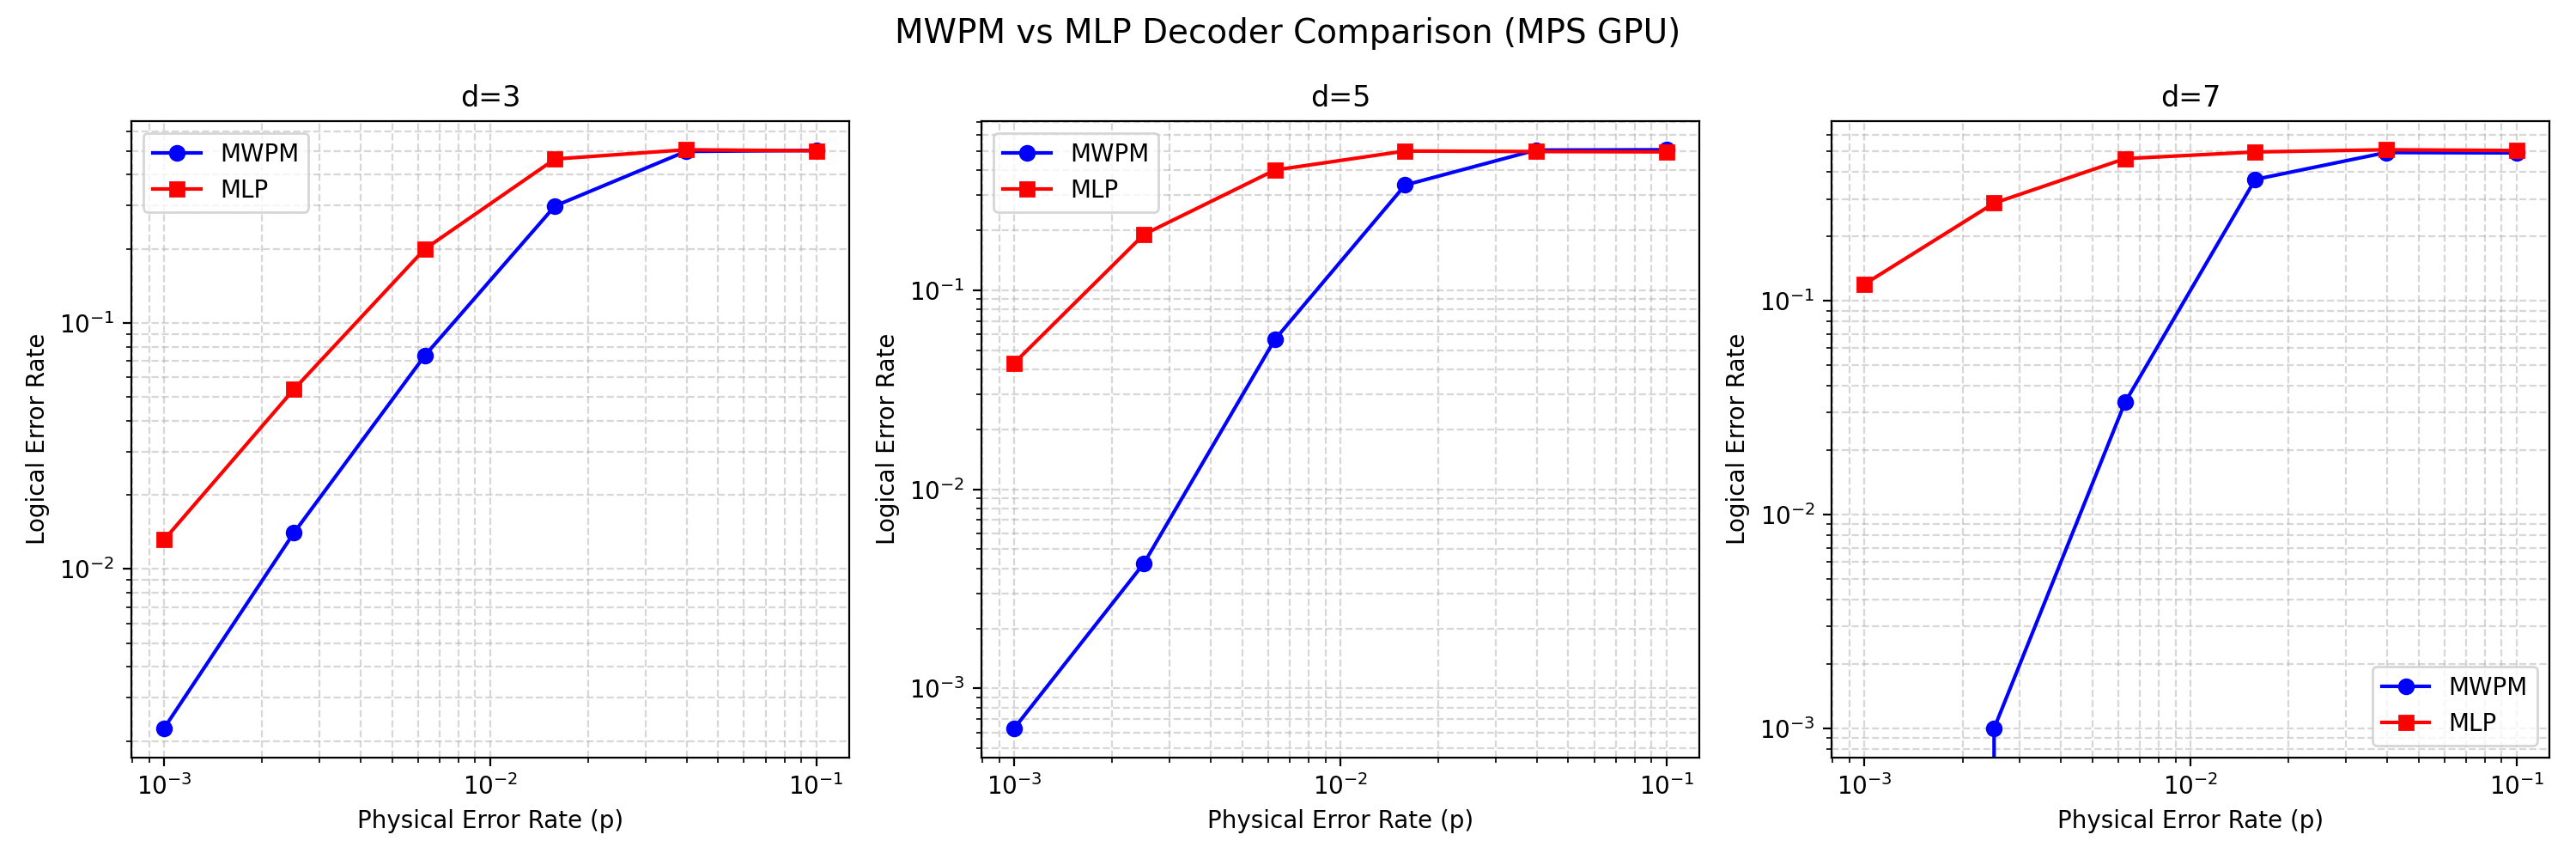
\includegraphics[width=0.9\textwidth]{../figures/decoder_comparison.png}
\caption{MLP vs MWPM logical error rates (MPS GPU accelerated).}
\label{fig:decoder}
\end{figure}

\subsection{Threshold Analysis}
Figure~\ref{fig:threshold} shows the extended threshold curves (d=3--11).

\begin{figure}[h]
\centering
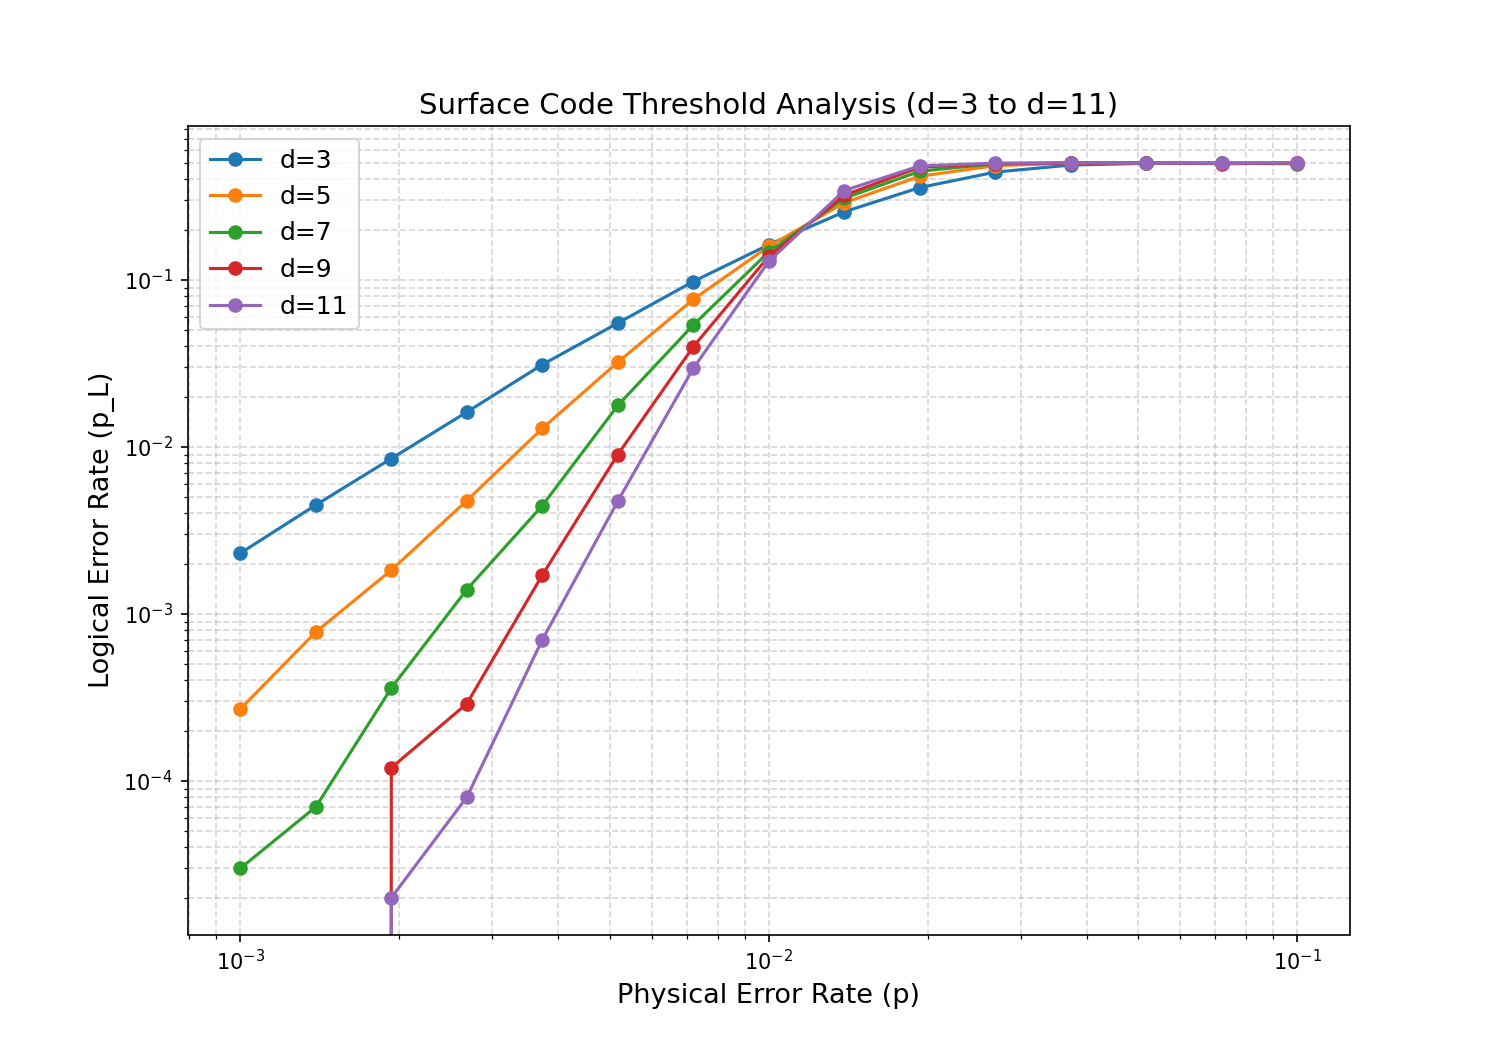
\includegraphics[width=0.9\textwidth]{../figures/threshold_plot_extended.png}
\caption{Surface-code threshold for distances 3--11.}
\label{fig:threshold}
\end{figure}

\end{document}

\subsection{Decoder Comparison}
Figure~\ref{fig:decoder} shows the MLP vs MWPM performance.

\begin{figure}[h]
\centering
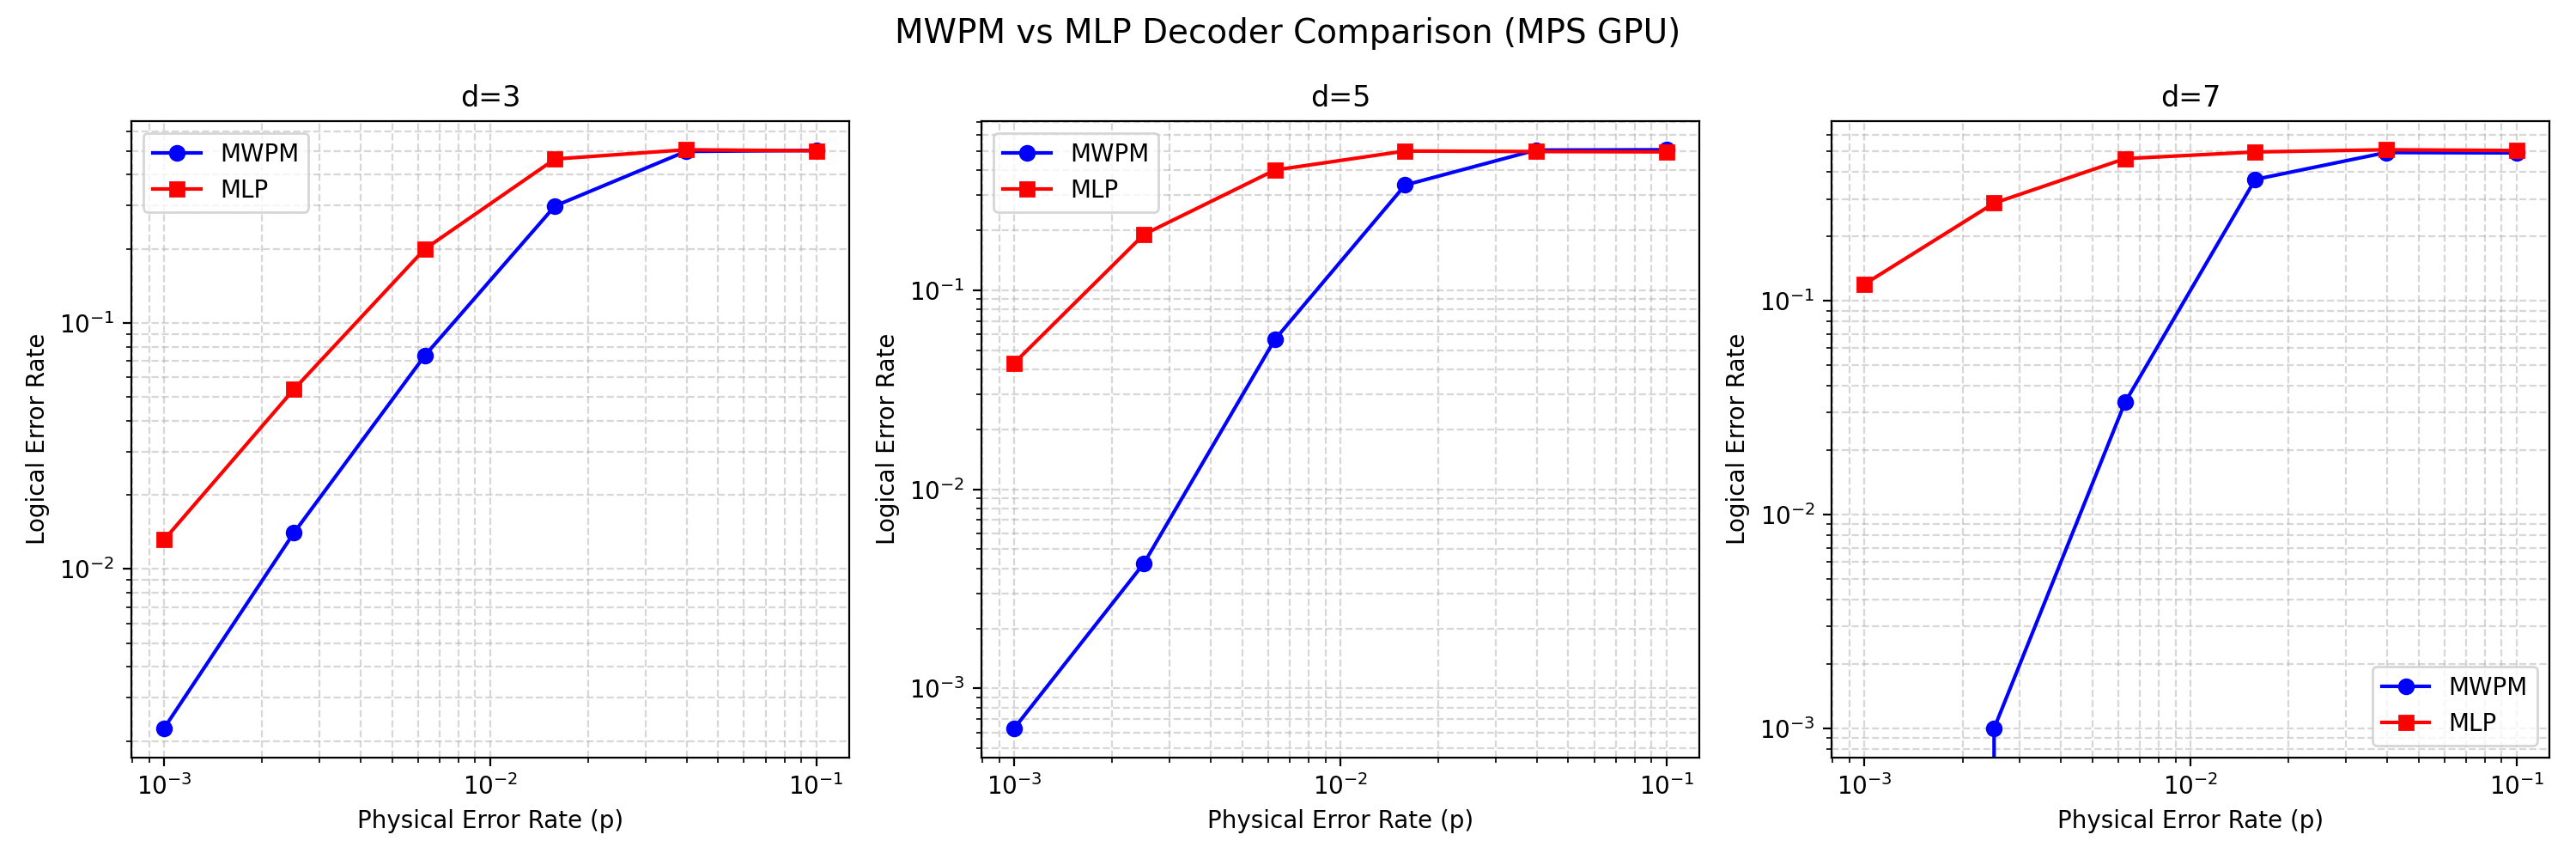
\includegraphics[width=0.9\textwidth]{../figures/decoder_comparison.png}
\caption{MLP vs MWPM logical error rates (MPS GPU accelerated).}
\label{fig:decoder}
\end{figure}

\subsection{Threshold Analysis}
Figure~\ref{fig:threshold} shows the extended threshold curves (d=3--11).

\begin{figure}[h]
\centering
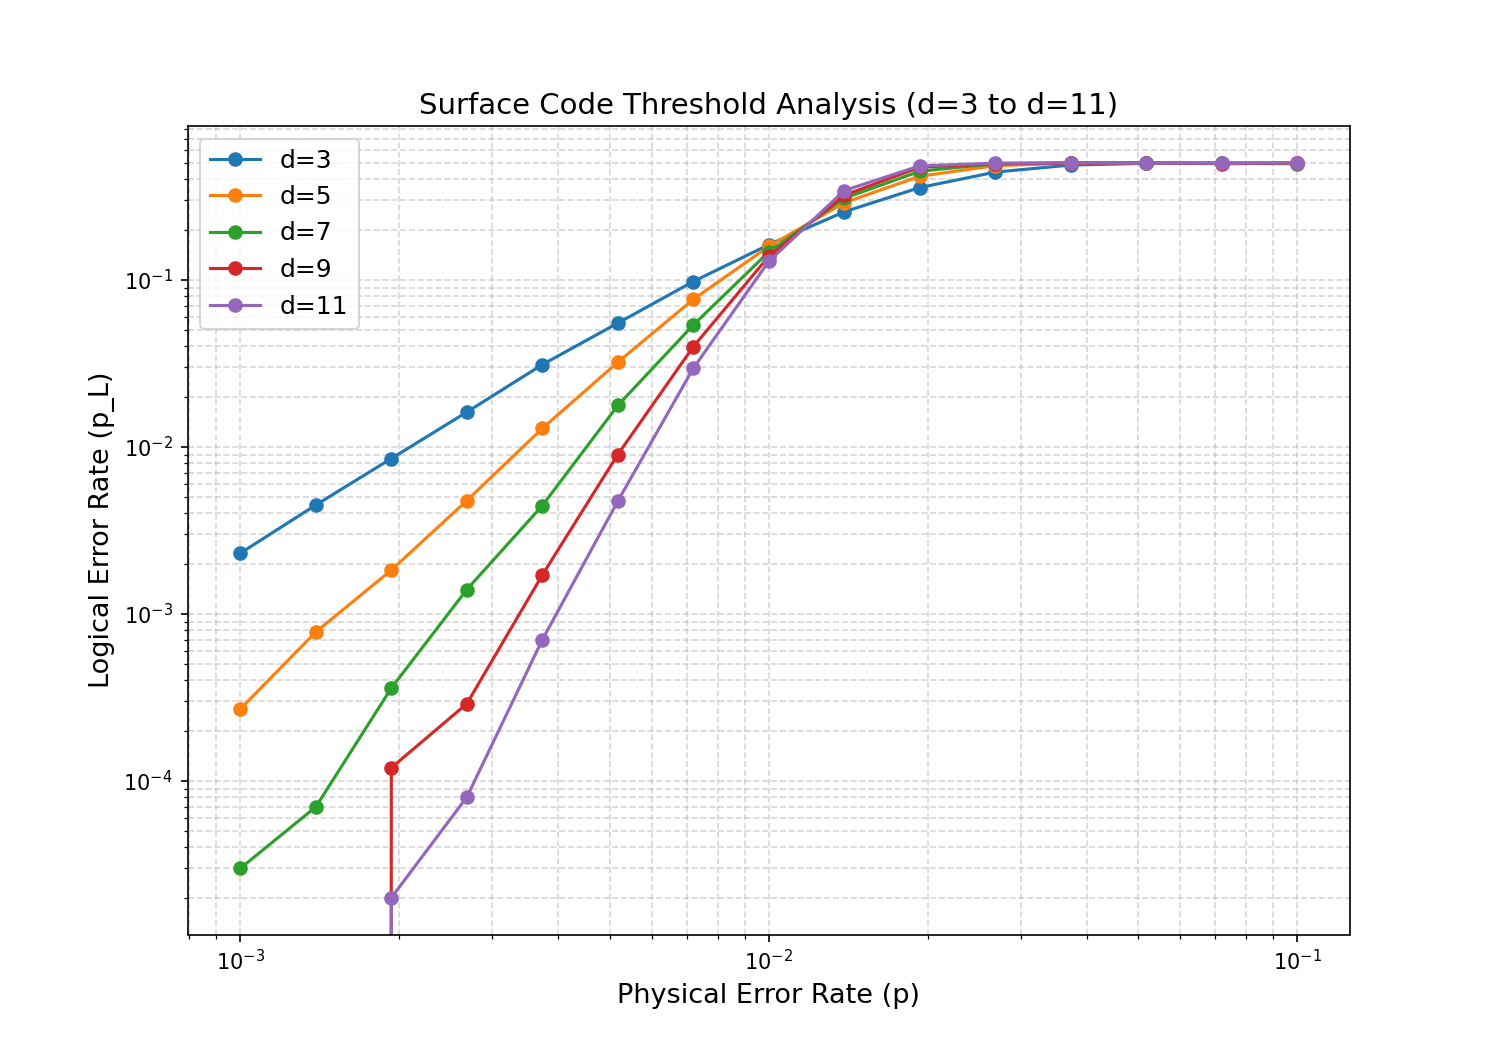
\includegraphics[width=0.9\textwidth]{../figures/threshold_plot_extended.png}
\caption{Surface-code threshold for distances 3--11.}
\label{fig:threshold}
\end{figure}

\end{document}
